\documentclass[pra,showpacs,priprent,twocolumn,superscriptaddress]{revtex4-1}
\usepackage{mathrsfs}
\usepackage{amsfonts}
\usepackage{amsmath}
\usepackage{txfonts}
\usepackage{amssymb}
\usepackage{graphicx}
\usepackage{bm}
\usepackage{color}
\usepackage[normalem]{ulem}
\newcommand{\R}[1]{{\color{red} #1}}
\newcommand{\B}[1]{{\color{blue} #1}}
\newcommand{\s}[2]{{{\color{red}{#1 }}{\color{blue}{\sout{#2}}}}}
\newcommand{\ket}[1]{|#1\rangle}
\newcommand{\bra}[1]{\langle #1|}
\newcommand{\Tr}{\text{Tr}}
\begin{document}
\title{Dark path holonomic qudit computation}
\author{Tomas Andr\'e}
\affiliation{Department of Physics and Astronomy, Uppsala University,
Box 516, Se-751 20 Uppsala, Sweden}
\author{Erik Sj\"oqvist}
\email{erik.sjoqvist@physics.uu.se}
\affiliation{Department of Physics and Astronomy, Uppsala University,
Box 516, Se-751 20 Uppsala, Sweden}
\date{\today}
\begin{abstract}
Non-adiabatic holonomic quantum computation (NHQC) is a method used to implement 
quantum gates with non-Abelian geometric phases. Due to high noise tolerance these phases 
can be used to construct resilient quantum gates. By using dark paths introduced for qubits 
in [Fundam. Res. {\bf X}, X (2022), doi:10.1016/j.fmre.2021.11.031], we show how to 
implement quantum gates for 
higher dimensional computation qudit elements instead. This gives higher parameter control 
compared to earlier implementations. We present a scheme that generalizes and achieves 
single-qudit universality using controllable high fidelity gates by including an auxiliary state. 
An explicit example is shown for the Qutrit. The scaling is linear in dimension and we show 
how any diagonal qudit gate can be implemented efficiently in any dimension.
\end{abstract}
\maketitle
\date{\today}

\section{Introduction}
The emerging field of quantum technology has many promising applications, one of them is quantum computation (QC), which currently is a very active area of research. Quantum computers make use of quantum mechanical effects such as superposition, entanglement, and interference to design powerful algorithms. These algorithms could be used to solve some hard problems which would not be  possible to solve using classical computation, such as efficient prime-number factoring \cite{shor94}. It can also be used to reduce the time complexity of some commonly used algorithms \cite{grover97}. Current quantum computers are very susceptible to decoherence and noise, and thus will not have any commercial use any time soon, but stand as an important proof of concept. 
The most common model for quantum computation is the circuit model, which is analogous to the classical circuits used for classical computers. Gates are replaced by unitary transformations (quantum gates) and bits by qubits. To achieve the computational advantage it is important to construct robust, noise-resilient quantum gates. A good candidate for this is holonomic quantum computation \cite{zanardi99,sjoqvist12}, which is based on the Berry phase \cite{berry84} and its non-Abelian and/or non-adiabatic generalizations \cite{aharonov87,anandan88,wilczek84}. These methods are only dependent on the geometry of the system and thus are resilient to local errors in the dynamical evolution.


The idea that elements of computation should be limited to two-dimensional qubits is sort of an arbitrary choice that most likely rose out of convenience due to binary logic. So why binary logic? It is simply the easiest non-trivial example, in binary things can be either $1$ or $0$, {\tt True} or {\tt False}, \textbf{on} or \textbf{off}. Due to its simplicity, it is no wonder that this is how the first computer was designed. But are we limited to bits? As early as 1840 a mechanical trenary (three-valued logic) calculation device was built by Thomas Fowler \cite{glusker05}, and in 1958 the first electronic trenary computer was built by the Soviet Union \cite{bursentsov11}. Even though it had many advantages over the binary computer it never saw the same widespread success. There is nothing in theory that forbids a higher dimensional computational basis, even more so when it comes to quantum computers, where the implementation of the elements of computation already surpasses the simplicity of \textbf{on} and \textbf{off}. There are promising qudit results that show potential, some are discussed in the review article \cite{wang20}, which gives a good overview of the field is given and further research into the topic is encouraged.

In this report we will show how to find a new geometric phase based scheme to implement qudits which could be more efficient than some current ones by making use of dark paths for increased parameter control and auxiliary states for increased fidelity. We do this by generalizing the idea of the scheme from \cite{ai22}. The report is structured as follows. The background section is split into two parts where the first part serves as a quick introduction to the most important aspects of quantum mechanics as well as the commonly used notation. Then follows a part more concerned with quantum computation, quantum information, and some of the more advanced quantum mechanical concepts that those are built upon. Then the main results are shown, first an explicit example for the qutrit and then how it generalizes in higher dimensions. The report ends with conclusions and a brief outlook.



\section{Dark path setting}

In \cite{ai22} a qubit is implemented by modifying the $\Lambda$ system, which is a 
pod-like system with one excited state and two ground states, adding an auxiliary state, 
effectively turning it into a tripod. The generalization to implement a qutrit is not trivial 
but it is clear that one extra ground state is required to make the computational basis 
larger. Another thing that is needed is to limit the number of dark states to one. The 
number of dark states is the difference between the number of excited states and the '
number of ground states \cite{shkolnikov20} (here the auxiliary state is not counted as 
a ground state). Therefore another excited state must be added as well. How these states are 
coupled is the hard part. We will see that the system given by the Hamiltonian in the Hilbert space $\{\ket{1},\ket{2},\ket{3},\ket{e_1},\ket{e_2},\ket{a}\}$

\begin{eqnarray}
\label{eq:Ham}
H = \sum_{j = 1}^2 \sum_{i =j}^{3} \omega_{ij}\ket{i}\bra{e_j}  + \frac{\Omega_{a}(t)}{2}\ket{a}\bra{e_2}  +\,\text{h.c.}
\end{eqnarray}
the system can be transformed into the dark-bright basis described in the new Hilbert space $\{\ket{1},\ket{2},\ket{3},\ket{e_1},\ket{e_2},\ket{a}\}$


\begin{eqnarray}
\label{eq:Ham_d}
H_d = \sum_{j = 1}^2 \frac{\Omega_j(t)}{2}e^{-i\phi_j}\ket{b_j}\bra{e_j}  + \frac{\Omega_a(t)}{2}\ket{a}\bra{e_2}  +\,\text{h.c.}
\end{eqnarray}
by rewriting it in terms of the basis kets:
\begin{eqnarray}
\label{eq:states}
\ket{d} & = & \cos\theta\ket{1} + e^{i\chi}\sin\theta\cos\varphi\ket{2} + 
e^{i\xi}\sin\theta\sin\varphi\ket{3},
\nonumber \\
\ket{b_1} & = & \frac{1}{\sqrt{1-\sin^2\theta\sin^2\varphi}} 
\left(-e^{-i\chi}\sin\theta\cos\varphi\ket{1} + \cos\theta\ket{2} \right),
\nonumber \\
\ket{b_2} & = & \frac{1}{\sqrt{1-\sin^2\theta\sin^2\varphi}} 
\bigg(\frac{1}{2}\sin 2\theta\sin\varphi\ket{1} 
\nonumber \\ 
 & & + \dfrac{e^{i\chi}}{2}\sin^2\theta\sin 2\varphi\ket{2} + 
 e^{i\xi}(\sin^2\theta\sin^2\varphi - 1)\ket{3}\bigg).
\end{eqnarray}
To obtain the original $\omega_{ij}$ parameters simply expand equation (\ref{eq:Ham_d}) in terms on the new kets from (\ref{eq:states}).

Now let us introduce two dark paths, $\ket{D_1(t)},\ket{D_2(t)}$. Along these paths the average energy is always zero, i.e $\bra{D_i(t)}H_d\ket{D_i(t)} = 0,\,i = 1,2$. Thus no dynamical phase is accumulated during the time evolution of these states and therefore follows the conditions required for NHQC. The following two states, parametrized by two angles $u(t), v(t)$, satisfy the dark path condition:
\begin{eqnarray}
\label{eq:dpaths}
\ket{D_1(t)} & = & \cos u e^{-i\phi_1}\ket{b_1} + i\sin u \ket{e_1},
\nonumber \\
\ket{D_2(t)} & = & \cos u\cos v e^{-i\phi_2}\ket{b_2} - i\sin u \ket{e_2} - \cos u\sin v \ket{a}.
\end{eqnarray}
It can easily be verified that $\bra{D_i(t)}H_d\ket{D_j(t)} = 0, i,j = 1,2$. The angles can be chosen so as to satisfy the constraint $\ket{D_i(0)}\bra{D_i(0)} = \ket{D_i(T)}\bra{D_i(T)}$, $i = 1,2$. This can be achieved by choosing $u(0) = u(T) = v(0) = v(T) = 0$. A valid choice is $u(t) = \frac{\pi}{2}\sin^2\frac{\pi t}{T}$ and $v(t) = \eta\left[1 - \cos u(t)\right]$, as for the qubit case \cite{ai22}. $\eta$ represents the coupling strength to the auxiliary state $\ket{a}$ and the system reverts into a tri-pod structure with two excited states when $\eta = 0$.
Each dark path starts in the respective bright state and travels along a curve and then returns to the bright state. Using the Schr{\"o}dinger equation one can reverse engineer the time dependent parameters $\Omega_i(t)$ by matching the factors in front of each state. A calculation yields 
\begin{eqnarray}
\Omega_1(t) &=& -2\dot{u},
 \nonumber \\ 
\Omega_2(t) &=& 2\left(\dot{v}\cot u\sin v + \dot{u}\cos v \right),
\nonumber \\
\Omega_a(t) &=& 2\left(\dot{v}\cot u\cos v - \dot{u}\sin v \right).
\end{eqnarray}


(oklart hur kapitlet ska avslutas här)
%\begin{figure}[h!]
%\centering
%\includegraphics[width=0.45\textwidth]{figurename.pdf}
%\caption{}
%\label{fig:figure_ref}
%\end{figure}

\section{Holonomic qudit gates}

\subsection{Qutrit $d=3$ gates} 
To construct a quantum gate, we make use of the method of multi-pulse single-loops \cite{herterich16}, for which the part of the time evolution operator that acts on the computational space is
\begin{eqnarray}
U_1 & = & \ket{d}\bra{d} -i\ket{e_1}\bra{b_1} -i\ket{e_2}\bra{b_2},\; \phi_1 = \phi_2 = 0,
\nonumber \\
U_2 & = & \ket{d}\bra{d} +ie^{i\gamma_1}\ket{b_1}\bra{e_1} +ie^{i\gamma_2}\ket{b_2}\bra{e_2},\; \phi_1 = -\gamma_1,\; \phi_2 = -\gamma_2
\end{eqnarray}
so the operator for one full loop is 
\begin{eqnarray}
\label{eq:trit-gate-1-loop}
U = U_2U_1 = \ket{d}\bra{d} + e^{i\gamma_1}\ket{b_1}\bra{b_1} + e^{i\gamma_2}\ket{b_2}\bra{b_2}.
\end{eqnarray}
This transformation can be parametrized by $6$ real parameters, $\chi,\xi,\theta,\varphi,\gamma_1,\gamma_2$, however it is not enough to construct all gates. For example $X_3$ requires 2 loops. The full gate is given by repeating $U$ with different set of parameters
\begin{eqnarray}
\label{eq:trit-gate-2-loop}
\mathbb{U} = U(\chi',\xi',\theta',\varphi',\gamma_1',\gamma_2') U(\chi,\xi,\theta,\varphi,\gamma_1,\gamma_2).
\end{eqnarray}
For $d = 3$, two loops are sufficient for universality, it can be used to parametrize the following gates: 
\begin{eqnarray}
X_3 &=& U(0,0,\dfrac{\pi}{4},\dfrac{\pi}{2},0,\pi)\times U(0,0,\dfrac{\pi}{2},\dfrac{\pi}{4},0,\pi) 
\nonumber\\&=& \begin{pmatrix}
0&0&1
\\
1&0&0
\\
0&1&0
\end{pmatrix},
\nonumber \\ 
Z_3 &=& U(0,0,0,0,\dfrac{2\pi}{3},\dfrac{4\pi}{3})
\nonumber\\&=& \begin{pmatrix}
1&0&0
\\
0&e^{\frac{2\pi i}{3}}&0
\\
0&0&e^{\frac{4\pi i}{3}}
\end{pmatrix},
\nonumber \\
T_3 &=& U(0,0,0,0,\dfrac{2\pi}{9},\dfrac{-2\pi}{9})
\nonumber\\&=& \begin{pmatrix}
1&0&0
\\
0&e^{\frac{2\pi i}{9}}&0
\\
0&0&e^{\frac{-2\pi i}{9}}
\end{pmatrix},
\nonumber\\
\text{H}_3 &=& U(6.41\cdot 10^{-4}, 6.56\cdot 10^{-4}, 0.48, 0.79, 1.58, 1.56) \nonumber\\&\times & U(9.81\cdot 10^{-3}, 0.00, 1.187, 2.15, 0.00, 1.57)
\nonumber\\&\approx & \dfrac{1}{\sqrt{3}}\begin{pmatrix}
1&1&1
\\
1&e^{\frac{2\pi i}{3}}&e^{\frac{4\pi i}{3}}
\\
1&e^{\frac{4\pi i}{3}}&e^{\frac{2\pi i}{3}}
\end{pmatrix}.
\end{eqnarray}
The set includes qutrit equivalents of the Hadamard and $T$-gate which constitutes a universal set. 

In FIG. \ref{fig:popH} and FIG. \ref{fig:popX} the population of the states during the H$_3$ and $X_3$ gates are shown.

\begin{figure}[h!]
\centering
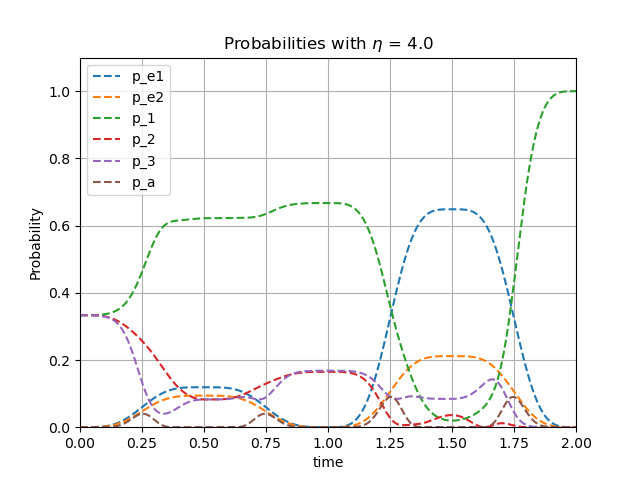
\includegraphics[width=0.45\textwidth]{pop_plot_H111.png}
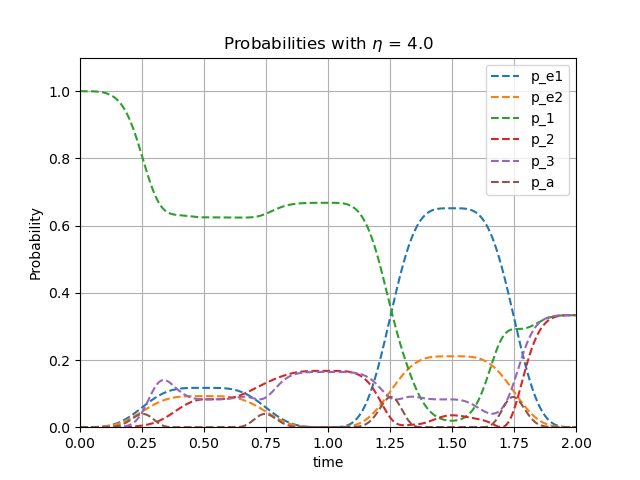
\includegraphics[width=0.45\textwidth]{pop_plot_H100.png}
\caption{The effect of the H$_3$-gate on the initial states $\dfrac{1}{\sqrt{3}}[1,1,1]$ (upper) and $[1,0,0]$ (lower). Note that since the plot shows the probabilities, phases cannot be seen in the plot.}
\label{fig:popH}
\end{figure}


\begin{figure}[h!]
\centering
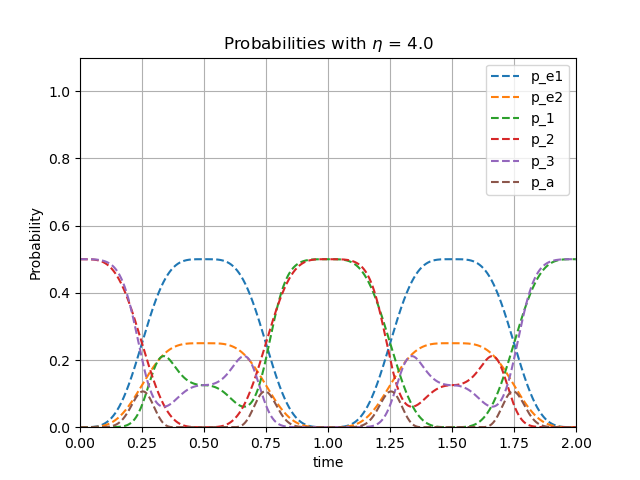
\includegraphics[width=0.45\textwidth]{pop_plot_X011.png}
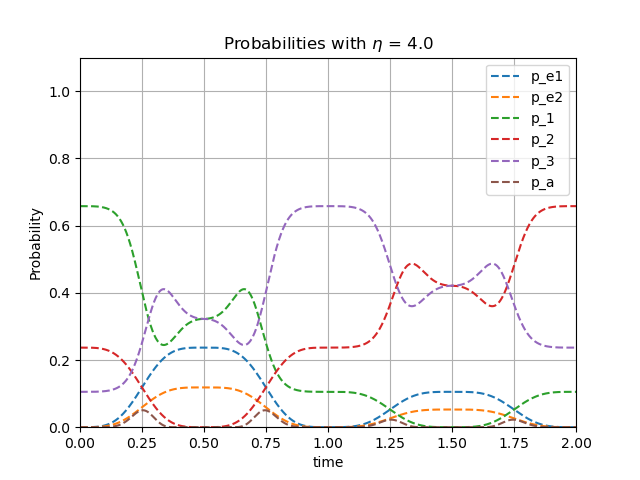
\includegraphics[width=0.45\textwidth]{pop_plot_X532.png}
\caption{The effect of the $X_3$-gate on the initial states $\dfrac{1}{\sqrt{2}}[0,1,1]$ (upper) and $\dfrac{1}{\sqrt{38}}[5,3,2]$ (lower). Note that since the plot shows the probabilities, phases cannot be seen in the plot.}
\label{fig:popX}
\end{figure}

All diagonal gates can be parametrized by a single loop by fixing $\theta = \varphi = \chi = \xi = 0$. The basis states reduce to $\ket{d} = \ket{1}, \ket{b_1} = \ket{2}, \ket{b_2} = -\ket{3}$. By equation (\ref{eq:trit-gate-1-loop}) it is possible to see that all diagonal unitaries can be specified by $\gamma_1$ and $\gamma_2$, up to a phase factor,
\begin{eqnarray}
U(0,0,0,0,\gamma_1,\gamma_2) = \begin{pmatrix}
1&0&0
\\
0&e^{i\gamma_1}&0
\\
0&0&e^{i\gamma_2}
\end{pmatrix}.
\end{eqnarray}

\subsection{Robustness test}
To assess the robustness of the gate the fidelity metric, $F$, is used, the metric measures how close two quantum states are to each other. Here we are only considering pure states, then the fidelity is: $F(\ket{\psi},\ket{\varphi}) = |\bra{\psi}\ket{\varphi}|$. The fidelity is averaged by sampling initial states and letting them evolve with time by numerically solving the Schrödinger equation using the SciPy implementation of backwards differentiation \cite{shampine97}. Then we introduce small shifts, $\Omega \mapsto \Omega(1 + \delta)$, for all $\Omega_i$ pulses in equation \ref{eq:Ham_d} and compare to the exact solution obtained by multiplying the gate with the initial state. The calculated fidelities are shown in FIG. \ref{fig:fidelity}. In the figures it can be seen that the coupling with the auxiliary state is more resilient to errors in the parameters than the original NHQC scheme. This is very similar to the results in 2 dimensions from \cite{ai22}, which suggests an improvement of robustness even in higher dimensions.

\begin{figure}[h!]
\centering
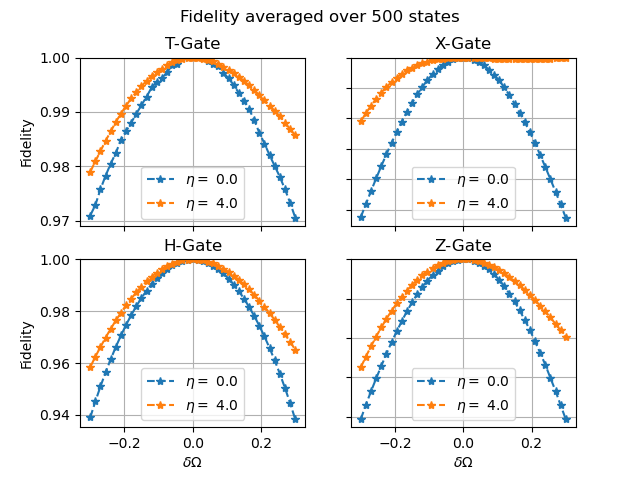
\includegraphics[width=0.45\textwidth]{Fid500.png}
\caption{Robustness test, average fidelity of the $T_3,X_3,Z_3,$ and H$_3$ gates. The averages are calculated by sampling over 500 randomized initial states with a perturbation of the $\Omega$-pulses, $\Omega \mapsto \Omega(1+\delta)$.}
\label{fig:fidelity}
\end{figure}

\subsection{Generalization} 
In the generalization $n$ will be used instead of the more common $d$ to refer to the dimension of a qudit. This is to avoid confusions with the dark states. To generalize the scheme for qudits with arbitrary dimension, $n$, the idea from the qutrit case can be extended: $n$ ground states, $m = n - 1$ excited states and 1 auxiliary state. The dimension of the Hilbert space is  $n + m + 1 = 2n + 1 -1 = 2n$. Once again the couplings are non-trivial and will be somewhat intricate, but the couplings given by the Hamiltonian in equation (\ref{eq:HamN}), will do the trick:

\begin{eqnarray}\label{eq:HamN}
H = \sum_{j = 1}^m \sum_{i = j}^n \omega_{ij} \ket{i}\bra{e_j} + \frac{\Omega_a(t)}{2}\ket{a}\bra{e_m} +\;\text{h.c}.
\end{eqnarray}

The general system for a qudit is given by $m$ excited states $\ket{e_i},\,i = 0,1,\dots,m$, $n$ ground states labeled $\ket{i},\,i = 1,2,\dots,n$ and one auxiliary state $\ket{a}$. The number of states always satisfies that $n-m = 1$ to limit the number of dark states to one \cite{shkolnikov20}.
The transitions occur only between excited states and ground states. The couplings follow a pattern; the first excited state $e_1$ is connected to all ground states, $e_2$ is connected to all ground states except $\ket{1}$, and so on. In general, the excited state $\ket{e_i}$ is connected to the $(n - i + 1)$ ground states with the largest indices. This holds for all excited states except the one with largest index, $i = m$, the excited state $\ket{e_m}$ is connected to the two highest labeled ground states and the auxiliary state $\ket{a}$. See equation (\ref{eq:HamN}) and Figure \ref{fig:HamN} for a clarification. 
From the standard basis $\{e_1,e_2,\dots,e_m,1,2,\dots,n,a\}$, it is possible to change to the dark-bright basis given by $\{e_1,e_2,\dots,e_m,b_1,b_2,\dots,b_{m},a,d\}$, in which the system is simpler to study. Assume there exists a dark state on the form 
\begin{eqnarray}
\ket{d} = c_1\ket{1} + c_2\ket{2} + c_3\ket{3} \dots + c_{n}\ket{n},\, |c_1|^2 + |c_2|^2 + \dots + |c_{n}|^2 = 1.
\end{eqnarray}
From this dark state one could define $n-1 = m$ bright states. Starting from $\ket{b_1}$, construct it such that it will be orthogonal to the dark state and all other bright states,
\begin{eqnarray}
\ket{b_1} = N_1\left(-c_2^{*}\ket{1} + c_1^{*}\ket{2}\right)
\end{eqnarray}
with $N_1$ being a normalization factor. Then choose additional bright states on the form
\begin{eqnarray}
\label{eq:birght_states}
\ket{b_2} &=& N_2 \left(c_1\ket{1} + c_2\ket{2} + \Lambda_3\ket{3}  \right),
\nonumber\\
\ket{b_3} &=&  N_3 \left(c_1\ket{1} + c_2\ket{2} + c_3\ket{3} + \Lambda_{4}\ket{4} \right),
\nonumber\\
&\vdots &
\nonumber\\
\ket{b_{m-1}} &=& N_{m-1} \left( c_1\ket{1} + c_2\ket{2} + \dots + c_{m-1}\ket{m-1}+ \Lambda_m\ket{m} \right),
\nonumber\\
\ket{b_{m}} &=& N_m \left( c_1\ket{1} + c_2\ket{2} + \dots + c_m\ket{m} + \Lambda_{m+1}\ket{m+1} \right).
\end{eqnarray}
By construction,  $\ket{b_1}$ is orthogonal to the dark state and all other bright states. For $k \geq 2$, $\ket{b_k}$ is $(k+1)$-dimensional, so it consists of $k+1$ basis-kets, where the coefficient, $\Lambda_{k+1}$ in front of the last ket is chosen such that $\ket{b_k}$ is orthogonal the dark state, $\ket{d}$. This will in turn make $\ket{b_k}$ orthonormal to any $\ket{b_{>k}}$ as they have the same states and coefficients as $\ket{d}$ for all the states involved in the inner product $\bra{b_{>k}}\ket{b_k} = \bra{d}\ket{b_k}$. Therefore, by choosing $\Lambda_k$ such that these inner products are zero, the construction will results in orthonormal states,  $\bra{b_i}\ket{b_j} = \delta_{ij}$. Explicitly for state $\ket{b_{k}}$, $k \geq 2$, the coefficient $\Lambda_{k+1}$ will be given by 
\begin{eqnarray}
\Lambda_{k+1} = -\dfrac{1}{c_{k+1}^{*}}\sum_{l = 1}^{k}|c_l|^2
\end{eqnarray}
and the normalization $N_{k}$ is given by 
\begin{eqnarray}
N_k =  \left( \sum_{l = 1}^k|c_l|^2  + \left|\Lambda_{k+1}\right|^2 \right)^{-1/2} = \left( \sum_{l = 1}^k|c_l|^2  + \left|-\frac{1}{c_{k+1}^{*}}\sum_{l = 1}^{k} |c_l|^2 \right|^2 \right)^{-1/2}.
\end{eqnarray}

The coefficients $c_i$ can be parametrized by the Euclidean components of the radius of the unit-$n$-sphere with an added phase factor.

\begin{eqnarray}
c_1 &=& \cos(\varphi_1),
\nonumber\\ 
c_2 &=& e^{i\theta_1}\sin(\varphi_1)\cos(\varphi_2),
\nonumber\\ 
c_3 &=& e^{i\theta_2}\sin(\varphi_1)\sin(\varphi_2)\cos(\varphi_3),
\nonumber\\
&\vdots &
\nonumber\\
c_{n-1} &=& e^{i\theta_{n-1}}\sin(\varphi_1)\dots\sin(\varphi_{n-2})\cos(\varphi_{n-1}),
\nonumber\\
c_{n} &=& e^{i\theta_{n}}\sin(\varphi_1)\dots\sin(\varphi_{n-2})\sin(\varphi_{n-1}).
\end{eqnarray}

In the dark-bright basis, the Hamiltonian can be written as
\begin{eqnarray}\label{eq:HamdN}
H_d = \sum_{i = 1}^m \frac{\Omega_i(t)}{2}e^{-i\phi_i}\ket{b_i}\bra{e_i} + \frac{\Omega_a(t)}{2}\ket{a}\bra{e_m} +\;\text{h.c}.
\end{eqnarray}
with $\Omega_i$ being real-valued time dependent parameters and the $\phi_i$ time independent phase factors. The explicit basis transformation $H \mapsto H_d$ is not that important but could be obtained by expanding the bright state kets into the standard basis from (\ref{eq:birght_states})

With this Hamiltonian $m$ independent dark paths can be constructed, and must satisfy $\bra{D_i(t)}H_d\ket{D_i(t)} = 0, i = 1,2,\dots,m$ and $\bra{D_i(t)}\ket{D_j(t)} = \delta_{ij}$. The dark paths can be parametrized by two functions $u(t),v(t)$ that satisfy the conditions $u(0) = v(0) = u(T) = v(T) = 0$ and  will have the form
\begin{eqnarray}
\ket{D_i(t)} &=& \cos u e^{-i\phi_i}\ket{b_i} + i\sin u \ket{e_i},\, i = 1,2,\dots,m-1,
\nonumber\\
\ket{D_m(t)} &=& \cos u \cos v e^{-i\phi_n}\ket{b_m} - i\sin u \ket{e_m} - \cos u \sin v \ket{a}.
\end{eqnarray}
The dark paths start in the bright state and travel along a curve where the expectation value of the energy is constantly $0$ and can thus be used for NHQC.

By using these states one can reverse engineer the Hamiltonian using the Schr{\"o}dinger equation to determine $\Omega_i$ and $\Omega_a$,
a calculation yields
\begin{eqnarray}
\Omega_1(t) &=& -2\dot{u},
\nonumber\\ 
\Omega_2(t) &=& -2\dot{u},
\nonumber\\
&\vdots &
\nonumber\\
\Omega_{m-1}(t) &=& -2\dot{u},
\nonumber\\
\Omega_m(t) &=& 2\left(\dot{v}\cot u\sin v + \dot{u}\cos v \right),
\nonumber\\
\Omega_a(t) &=& 2\left(\dot{v}\cot u\cos v - \dot{u}\sin v \right).
\end{eqnarray}

The time evolution is split into $k$ loops, each loop with two pulses \cite{herterich16}, $0 \longrightarrow T/2$ and $T/2 \longrightarrow T$. The relevant part of the time evolution operator for one loop is  
\begin{eqnarray}
U_1(T/2,0) = \ket{d}\bra{d} -i\sum_{i = 1}^m \ket{e_i}\bra{b_i},\, \phi_i = 0, i = 1,2,\dots,n,
\end{eqnarray} and 
\begin{eqnarray}
U_2(T,T/2) = \ket{d}\bra{d} + i\sum_{i = 1}^m e^{i\gamma_i}\ket{b_i}\bra{e_i},\, \phi_i = 0, i = 1,2,\dots,n.
\end{eqnarray}
The full operator for one loop is then given by 
\begin{eqnarray}
U(T,0) = U_2U_1 = \ket{d}\bra{d} + \sum_{i = 1}^{m}e^{i\gamma_i}\ket{b_i}\bra{b_i}.
\end{eqnarray}
It is clear that $U$ is unitary in the subspace $\{d,b_1,b_2,\dots, b_n\}.$ The unitary is parametrized by $3m = 3(n-1)$ parameters for $ n\geq 2$,
\begin{eqnarray}
U(\varphi_1,\dots,\varphi_m,\theta_1,\dots,\theta_m,\gamma_1,\dots,\gamma_m).
\end{eqnarray} 
Applying the unitary with different parameters in sequence up to $k$ times is enough to create any desirable gate $\mathbb{U} = U^k$. The unitary is controlled by $3(n-1)$ parameters while $n$ dimensional qudit has more degrees of freedom than covered with a single loop.

The qudit state space of dimension $n$ is equivalent to that of the special unitary group, $SU(n)$, which has dimensionality $\dim(SU(n)) = n^2 -1$. To cover all degrees of freedom, $k$ must satisfy $3(n-1)k \geq n^2 -1$, which require $k \geq \frac{n+1}{3}$. Thus the number of loops needed to create any unitary scales linearly at worst since some gates can be created with fewer loops. 

In the case of equality $k =\frac{n+1}{3}$, when $n = 3j + 2,\, j \in \mathbb{N}$, the fewest amount of loops per dimension is achieved and could potentially be more efficient carriers of information since the same number of loops must be carried out while higher dimension has higher information capacity.

The scaling of the qudit gate is linear at worst both in the number of loops and in the number of parameters needed for control. In fact, any diagonal gate only requires one loop: by setting $\varphi_1 = \dots = \varphi_m = \theta_1 = \dots = \theta_m = 0$ the unitary reduces to the form
\begin{eqnarray}
\label{eq:diagate}
U(0,\dots,0,\gamma_1,\dots,\gamma_m) = \ket{1}\bra{1} + \sum_{k = 2}^n e^{i\gamma_k}\ket{k}\bra{k}.
\end{eqnarray}
The effect of this variable choice makes $c_1 = 1, c_{i\neq 1} = 0$. By (\ref{eq:birght_states}) the only thing not obvious is how this affects the $\Lambda$ coefficients.
For the state $\ket{b_k}$, $k \geq 3$, fixing $c_1 = 1$ and letting all other states approach $0$ yields:
\begin{eqnarray}
\lim_{c_{i\neq 1} \rightarrow 0} \ket{b_k} &=& \lim_{c_{i\neq 1} \rightarrow 0}\frac{1}{N_k}\Lambda_{k+1} \ket{k+1} \nonumber \\
&=& \lim_{c_{i\neq 1} \rightarrow 0} \left(1  + \left|-\frac{1}{c_{k+1}^{*}}\right|^2 \right)^{-1/2}\left(-\frac{1}{c_{k+1}^{*}}\right) \ket{k+1} \nonumber\\
&=& \lim_{c_{i\neq 1} \rightarrow 0} \left|-\frac{1}{c_{k+1}^{*}}\right|^{-1}\left(-\frac{1}{c_{k+1}^{*}}\right) \ket{k+1} \nonumber\\
&=& -\ket{k+1}.
\end{eqnarray}
Therefore $\ket{d} = \ket{1}, \ket{b_1} = \ket{2}, \ket{b_2} = -\ket{3}, \ket{b_3} = -\ket{4}, \dots, \ket{b_m} = -\ket{m+1}$, and thus the unitary will take the form (\ref{eq:diagate}) so any diagonal unitary can be created up to an overall phase. 

\section{Conclusions}
We have shown how to explicitly create a quantum mechanical system, which could be used to emulate a qutrit and corresponding single-qutrit gates. This is done by expanding the dark path qubit scheme \cite{ai22} into a higher dimension. We have shown how it will generalize in the qudit case and using auxiliary states to improve the robustness of the gates. Universality for the qutrit can be obtained using the Hadamard and $T$ gates in 3 dimensions. The qutrit gates have a high fidelity and their robustness is improved by the inclusion of the auxiliary state in a similar way as for the qubit [15], which suggests that this method can be beneficial for higher dimensional qudits to improve robustness. In the general case for the qudit we have also shown how any dimensional single-qudit diagonal unitary could be created by a single multi-pulse loop in parameter space and that non-diagonal unitaries scale linearly at worst in the number of loops and parameters required for control of each loop scale linearly. The possibility that the scheme expands efficiently into certain prime dimension have been discussed.

\section{Acknowledgment}
E.S. acknowledges financial support from the Swedish Research Council (VR) through 
Grant No. 2017-03832.


\begin{thebibliography}{99}
\bibitem{zanardi99} P. Zanardi and M. Rasetti,  
Holonomic quantum computation, 
Phys. Lett. A {\bf 264}, 94 (1999). 

\bibitem{sjoqvist12} E. Sj\"{o}qvist, D. M. Tong, L. M. Andersson, B. Hessmo, M. Johansson,
and K. Singh, 
Non-adiabatic holonomic quantum computation, 
New J. Phys. {\bf 14}, 103035 (2012).

\bibitem{wilczek84} F. Wilczek and A. Zee, 
Appearance of Gauge Structure in Simple Dynamical Systems, 
Phys. Rev. Lett. {\bf 52}, 2111  (1984).

\bibitem{anandan88} J. Anandan, 
Non-adiabatic non-Abelian geometric phase, 
Phys. Lett. A {\bf 133} 171 (1988). 

\bibitem{duan01} L.-M. Duan, J. I. Cirac, and P. Zoller, 
Geometric Manipulation of Trapped Ions for Quantum Computation, 
Science {\bf 292}, 1695 (2001). 

\bibitem{herterich16} E. Herterich and E. Sj\"oqvist,  
Single-loop multiple-pulse nonadiabatic holonomic quantum gates, 
Phys. Rev. A {\bf 94}, 052310 (2016). 

\bibitem{wang20} Y. Wang, Z. Hu, B. C. Sanders, and S. Kais,  
Qudits and High-Dimensional Quantum Computing, 
Front. Phys. {\bf 8}, 589504 (2020). 

\bibitem{ai22} M. Z. Ai, S. Li, R. He, Z. Y. Xue, J. M. Cui, Y. F. Huang, C. F. Li and G. C. Guo, 
Experimental Realization of Nonadiabatic Holonomic Single-Qubit Quantum Gates with 
Two Dark Paths in a Trapped Ion, 
Fundam. Res. (2022). 

\bibitem{shkolnikov20} V. O. Shkolnikov and G. Burkard, 
Effective Hamiltonian theory of the geometric evolution of quantum systems, 
Phys. Rev. A {\bf 101}, 042101 (2020). 

\bibitem{morris83} J.R.Morris and B. W. Shore, 
Reduction of degenerate two-level excitation to independent two-state system, 
Phys. Rev. A {\bf 27}, 906 (1983).

\bibitem{aharonov87} Y. Aharonov and J. Anandan, 
Phase change during a cyclic quantum evolution, 
Phys. Rev. Lett. {\bf 58}, 1593 (1987). 

\bibitem{shor94} P. W. Shor, Algorithms for quantum computation: discrete logarithms and factoring in \textit{35th Proceedings Annual Symposium on Foundations of Computer Science}, pp. 124-134 (1994).


\bibitem{grover97} L. K. Grover, Quantum Mechanics Helps in Searching for a Needle in a Haystack, Phys. Rev. Lett. \textbf{79}, 325 (1997).

\bibitem{berry84} M. V. Berry, Quantal phase factors accompanying adiabatic changings, Proc. Roy. Soc. London Ser. A \textbf{392}, 45 (1984).

\bibitem{glusker05} M. Glusker, D. M. Hogan and P. Vass, The ternary calculating machine of Thomas Fowler, IEEE Annals of the History of Computing \textbf{27}, 4 (2005).

\bibitem{bursentsov11} N. P. Brusentsov and J. Ramil Alvarez, Ternary Computers: The Setun and the Setun 70, \textbf{357}, 74 (2011).


\bibitem{shampine97} L. F. Shampine and M. W. Reichelt, The MATLAB ODE Suite, SIAM journal on scientific computing \textbf{18}, 1 (1997).

\end{thebibliography}
\end{document}